% Options for packages loaded elsewhere
\PassOptionsToPackage{unicode}{hyperref}
\PassOptionsToPackage{hyphens}{url}
%
\documentclass[
  english,
  man,mask,floatsintext]{apa6}
\usepackage{amsmath,amssymb}
\usepackage{lmodern}
\usepackage{ifxetex,ifluatex}
\ifnum 0\ifxetex 1\fi\ifluatex 1\fi=0 % if pdftex
  \usepackage[T1]{fontenc}
  \usepackage[utf8]{inputenc}
  \usepackage{textcomp} % provide euro and other symbols
\else % if luatex or xetex
  \usepackage{unicode-math}
  \defaultfontfeatures{Scale=MatchLowercase}
  \defaultfontfeatures[\rmfamily]{Ligatures=TeX,Scale=1}
\fi
% Use upquote if available, for straight quotes in verbatim environments
\IfFileExists{upquote.sty}{\usepackage{upquote}}{}
\IfFileExists{microtype.sty}{% use microtype if available
  \usepackage[]{microtype}
  \UseMicrotypeSet[protrusion]{basicmath} % disable protrusion for tt fonts
}{}
\makeatletter
\@ifundefined{KOMAClassName}{% if non-KOMA class
  \IfFileExists{parskip.sty}{%
    \usepackage{parskip}
  }{% else
    \setlength{\parindent}{0pt}
    \setlength{\parskip}{6pt plus 2pt minus 1pt}}
}{% if KOMA class
  \KOMAoptions{parskip=half}}
\makeatother
\usepackage{xcolor}
\IfFileExists{xurl.sty}{\usepackage{xurl}}{} % add URL line breaks if available
\IfFileExists{bookmark.sty}{\usepackage{bookmark}}{\usepackage{hyperref}}
\hypersetup{
  pdftitle={No meaningful effects of COVID-19 related social media use on well-being},
  pdflang={en-EN},
  pdfkeywords={COVID-19, Coronavirus, well-being, affect, life satisfaction, social media use, news use, communication, random effects within between model, panel study, longitudinal.},
  hidelinks,
  pdfcreator={LaTeX via pandoc}}
\urlstyle{same} % disable monospaced font for URLs
\usepackage{graphicx}
\makeatletter
\def\maxwidth{\ifdim\Gin@nat@width>\linewidth\linewidth\else\Gin@nat@width\fi}
\def\maxheight{\ifdim\Gin@nat@height>\textheight\textheight\else\Gin@nat@height\fi}
\makeatother
% Scale images if necessary, so that they will not overflow the page
% margins by default, and it is still possible to overwrite the defaults
% using explicit options in \includegraphics[width, height, ...]{}
\setkeys{Gin}{width=\maxwidth,height=\maxheight,keepaspectratio}
% Set default figure placement to htbp
\makeatletter
\def\fps@figure{htbp}
\makeatother
\setlength{\emergencystretch}{3em} % prevent overfull lines
\providecommand{\tightlist}{%
  \setlength{\itemsep}{0pt}\setlength{\parskip}{0pt}}
\setcounter{secnumdepth}{-\maxdimen} % remove section numbering
% Make \paragraph and \subparagraph free-standing
\ifx\paragraph\undefined\else
  \let\oldparagraph\paragraph
  \renewcommand{\paragraph}[1]{\oldparagraph{#1}\mbox{}}
\fi
\ifx\subparagraph\undefined\else
  \let\oldsubparagraph\subparagraph
  \renewcommand{\subparagraph}[1]{\oldsubparagraph{#1}\mbox{}}
\fi
% Manuscript styling
\usepackage{upgreek}
\captionsetup{font=singlespacing,justification=justified}

% Table formatting
\usepackage{longtable}
\usepackage{lscape}
% \usepackage[counterclockwise]{rotating}   % Landscape page setup for large tables
\usepackage{multirow}		% Table styling
\usepackage{tabularx}		% Control Column width
\usepackage[flushleft]{threeparttable}	% Allows for three part tables with a specified notes section
\usepackage{threeparttablex}            % Lets threeparttable work with longtable

% Create new environments so endfloat can handle them
% \newenvironment{ltable}
%   {\begin{landscape}\begin{center}\begin{threeparttable}}
%   {\end{threeparttable}\end{center}\end{landscape}}
\newenvironment{lltable}{\begin{landscape}\begin{center}\begin{ThreePartTable}}{\end{ThreePartTable}\end{center}\end{landscape}}

% Enables adjusting longtable caption width to table width
% Solution found at http://golatex.de/longtable-mit-caption-so-breit-wie-die-tabelle-t15767.html
\makeatletter
\newcommand\LastLTentrywidth{1em}
\newlength\longtablewidth
\setlength{\longtablewidth}{1in}
\newcommand{\getlongtablewidth}{\begingroup \ifcsname LT@\roman{LT@tables}\endcsname \global\longtablewidth=0pt \renewcommand{\LT@entry}[2]{\global\advance\longtablewidth by ##2\relax\gdef\LastLTentrywidth{##2}}\@nameuse{LT@\roman{LT@tables}} \fi \endgroup}

% \setlength{\parindent}{0.5in}
% \setlength{\parskip}{0pt plus 0pt minus 0pt}

% Overwrite redefinition of paragraph and subparagraph by the default LaTeX template
% See https://github.com/crsh/papaja/issues/292
\makeatletter
\renewcommand{\paragraph}{\@startsection{paragraph}{4}{\parindent}%
  {0\baselineskip \@plus 0.2ex \@minus 0.2ex}%
  {-1em}%
  {\normalfont\normalsize\bfseries\itshape\typesectitle}}

\renewcommand{\subparagraph}[1]{\@startsection{subparagraph}{5}{1em}%
  {0\baselineskip \@plus 0.2ex \@minus 0.2ex}%
  {-\z@\relax}%
  {\normalfont\normalsize\itshape\hspace{\parindent}{#1}\textit{\addperi}}{\relax}}
\makeatother

% \usepackage{etoolbox}
\makeatletter
\patchcmd{\HyOrg@maketitle}
  {\section{\normalfont\normalsize\abstractname}}
  {\section*{\normalfont\normalsize\abstractname}}
  {}{\typeout{Failed to patch abstract.}}
\patchcmd{\HyOrg@maketitle}
  {\section{\protect\normalfont{\@title}}}
  {\section*{\protect\normalfont{\@title}}}
  {}{\typeout{Failed to patch title.}}
\makeatother
\keywords{COVID-19, Coronavirus, well-being, affect, life satisfaction, social media use, news use, communication, random effects within between model, panel study, longitudinal.}
\usepackage{lineno}

\linenumbers
\usepackage{csquotes}
\setlength{\parskip}{0em}
\raggedbottom
\note{\clearpage}
\ifxetex
  % Load polyglossia as late as possible: uses bidi with RTL langages (e.g. Hebrew, Arabic)
  \usepackage{polyglossia}
  \setmainlanguage[]{english}
\else
  \usepackage[main=english]{babel}
% get rid of language-specific shorthands (see #6817):
\let\LanguageShortHands\languageshorthands
\def\languageshorthands#1{}
\fi
\ifluatex
  \usepackage{selnolig}  % disable illegal ligatures
\fi
\newlength{\cslhangindent}
\setlength{\cslhangindent}{1.5em}
\newlength{\csllabelwidth}
\setlength{\csllabelwidth}{3em}
\newenvironment{CSLReferences}[2] % #1 hanging-ident, #2 entry spacing
 {% don't indent paragraphs
  \setlength{\parindent}{0pt}
  % turn on hanging indent if param 1 is 1
  \ifodd #1 \everypar{\setlength{\hangindent}{\cslhangindent}}\ignorespaces\fi
  % set entry spacing
  \ifnum #2 > 0
  \setlength{\parskip}{#2\baselineskip}
  \fi
 }%
 {}
\usepackage{calc}
\newcommand{\CSLBlock}[1]{#1\hfill\break}
\newcommand{\CSLLeftMargin}[1]{\parbox[t]{\csllabelwidth}{#1}}
\newcommand{\CSLRightInline}[1]{\parbox[t]{\linewidth - \csllabelwidth}{#1}\break}
\newcommand{\CSLIndent}[1]{\hspace{\cslhangindent}#1}

\title{No meaningful effects of COVID-19 related social media use on well-being}
\author{Blinded for review\textsuperscript{1}}
\date{}


\shorttitle{COVID-19 related social media use and well-being}

\authornote{

Blinded for review.

Correspondence concerning this article should be addressed to Blinded for review, Blinded for review. E-mail: Blinded for review

}

\affiliation{\vspace{0.5cm}\textsuperscript{1} Blinded for review}

\abstract{
In times of crisis such as the Corona pandemic, it is important that citizens stay informed about recent events, the latest political decisions, or mandatory protection measures. To this end, many people use various types of media, and increasingly social media. However, because social media are particularly engaging, some find it hard to disconnect and cannot stop `doomscrolling.' In this preregistered study, I investigate whether using social media for COVID-19 related topics might put personal well-being at risk. To answer this question I analyzed data from the Austrian Corona Panel Project, which consists of 24 waves with overall 3,018 participants. I ran three random effects cross lagged panel models, controlling for several stable and varying covariates. Results showed that the effects of various types of COVID-19 related social media use on several indicators of well-being were very small, arguably too small to matter. The findings suggest fears that social media use during times of crisis might be detrimental for well-being are likely to be unfounded.
}



\begin{document}
\maketitle

During the COVID-19 pandemic,
numerous events unfolded in quick succession.
Several open questions emerged.
How dangerous is the virus?
Is it spreading in my region?
How is it transmitted?
How can I protect myself?
Because for many it was (and continues to be) a matter of life or death, citizens had to stay informed regarding the latest developments.
Governments around the world implemented safety measures, ranging from wearing masks, keeping physical distance, to complete lockdowns.
In this extraordinary situation, people used media excessively to attain information, and especially social media were at an all time high (Statista, 2021).
A new phenomenon termed ``doomscrolling'' emerged:
People could not stop using social media to learn about COVID-19 related news.

Several people reported that they were glued to their screens and could not pursue other relevant activities such as working, taking a break, or even child-care (Klein, 2021).
As doomscrolling increased it became doubtful whether such a surge in social media use could still be considered useful and adaptive, or whether it created an additional hazard for users' mental health (Sandstrom, Buchanan, Aknin, \& Lotun, 2021).
These concerns seem justified: A study with 6,233 people from Germany found that ``{[}f{]}requency, duration and diversity of media exposure were positively associated with more symptoms of depression and unspecific and COVID-19 specific anxiety'' (Bendau et al., 2021), which implies negative consequences for well-being.

As a result, with this study I want to build on this research and investigate the question whether COVID-19 related social media use during the pandemic affected well-being.
To this end, I analyze a large-scale panel study from the Austrian Corona Panel Project (Kittel et al., 2020).
The panel consists of 24 waves and has an overall sample size of 3018.
At least 1,500 participants took part per wave, and the sample is representative of the Austrian population.
The panel study collected a large number of variables.
Being able to control for many confounding third variables, both stable and varying, and together with the longitudinal design, this creates a unique opportunity to investigate the causal effects of COVID-19 related social media use on well-being.

\hypertarget{defining-well-being-and-media-use}{%
\subsection{Defining Well-being and Media Use}\label{defining-well-being-and-media-use}}

The underlying theories that guided the selection of variables for this study are the two-continua model of mental health (Greenspoon \& Saklofske, 2001) and the hierarchical taxonomy of computer-mediated medation (Meier \& Reinecke, 2020).
According to the two-continua model, mental health consists of two dimensions: psychopathology and well-being.
Well-being can be further differentiated into subjective and psychological well-being (Diener, Lucas, \& Oishi, 2018).
Whereas subjective well-being emphasizes hedonic aspects such as happiness and joy, psychological well-being focuses on eudaimonic aspects like fulfillment and meaning.
Subjective well-being is primarily about achieving positive affect and avoiding negative affect.
One of the most prominent indicators of well-being is life satisfaction.
In my view, life satisfaction should be considered a meta concept that combines psychological and subjective well-being, because it represents a general appraisal of one's life.
Notably, life satisfaction is stable and fluctuates only little, whereas it's the exact opposite for affect (Dienlin \& Johannes, 2020).
To capture well-being in this study, I thus build on life satisfaction, positive affect, and negative affect.
Together, this should provide an encompassing perspective on potential media effects.

The hierarchical taxonomy of computer-mediated communication differentiates six levels of how people engage with digital technology.
First, the device (e.g., smartphone); second, the type of application (e.g., social networking site); third, the branded application (e.g., Twitter); fourth, the feature (e.g., status post); fifth, the interaction (e.g., one-to-many); sixth, the message (e.g., content) (Meier \& Reinecke, 2020).
Whereas the first four levels are focused on the \emph{channel}, the last two address the \emph{type} of communication.
To measure social media use for consumption of COVID-19 related news and topics, I here employ both the channel and the communication perspective, which together should provide a more nuanced understanding of communication.

First, I will investigate how different types of communication affect well-being.
Specifically, I will differentiate between active and passive use.
I will distinguish (a) \emph{reading} COVID-19 related social media news (passive), \emph{posting} content regarding COVID (active), and \emph{liking and sharing} COVID-19 related posts (both active and passive).
Second, I will analyze also how using the most prominent branded applications affect well-being, and whether this effect changes across applications.
According to Meier and Reinecke (2020), branded apps are separate entities with different effects.
Therefore, Twitter might have a different effect than WhatsApp because of their different affordances.
For example, Waterloo, Baumgartner, Peter, and Valkenburg (2018) found that it is more adequate to express negative emotions on WhatsApp than on Twitter or on Instagram.
The branded applications investigated here are Facebook, Twitter, Instagram, WhatsApp, and YouTube.
Worth noting, this study is not about \emph{general} social media during times of COVID, but on social media use \emph{focused} on COVID-19 related news and interactions.
Examples of such media use include posting about the pandemic or retweeting COVID-19 related posts.

\hypertarget{effects-of-social-media-on-well-being}{%
\subsection{Effects of Social Media on Well-Being}\label{effects-of-social-media-on-well-being}}

So far, there is only little empirical research on COVID-19 related social media use and well-being.
In their study on the relations between media use and mental health during the pandemic, Bendau et al. (2021) found that people who used social media as a primary source of information reported on average ``significantly more unspecific anxiety and depression {[}{]} and significantly more specific COVID-19 related anxiety symptoms'' (p.~288).
Hence, this might hint at potential negative effects of social media as news use.
However, note that this finding comes from a between-person relation stemming from cross-sectional data (see below).
We, therefore, don't know whether the differences in mental health and well-being are due to social media use or other third variables, such as age, health, or education.
Eden, Johnson, Reinecke, and Grady (2020) analyzed the media use of 425 US college students during the first wave of the pandemic, and found both positive and negative relations with well-being.
In a sample of 312 respondents collected via Amazon Mechanical Turk, Choi and Choung (2021) reported that people who used media to attain information were more lonely and less satisfied with their lives.
Stainback, Hearne, and Trieu (2020) analyzed a large-scale study with 11,537 respondents from the US and found that increased COVID-19 media consumption was related to more psychological distress.

On the other hand, the question of whether and how \emph{general} social media use affect well-being is well-researched.
This also holds true for the different types of communication such as active or passive use.
A meta review (i.e., an analysis of meta-analyses), found that the relation between social media use and well-being is likely in the negative spectrum but very small, potentially too small to matter (Meier \& Reinecke, 2020).
What determines whether an effect is considered trivial or small?
If we refer to standardized effect sizes, according to Cohen (1992) small effect sizes start at \emph{r} = .10.
And indeed, several if not most of the current meta-analyses find effect sizes below that threshold (Ferguson et al., 2021; Huang, 2017; Meier \& Reinecke, 2020).

These overviews are well aligned with several individual new studies that employed advanced methods (Keresteš \& Štulhofer, 2020; Orben, Dienlin, \& Przybylski, 2019; Przybylski, Nguyen, Law, \& Weinstein, 2021; Schemer, Masur, Geiß, Müller, \& Schäfer, 2021).
For example, Beyens, Pouwels, Driel, Keijsers, and Valkenburg (2021) reported that although for some users (roughly one quarter) the effects were negative, for almost the same number of users they were positive, while for the majority the effects were neutral.
In conclusion, most effects are somewhere between trivial and small.
I therefore think it's most convincing to expect trivial to small effects also in the case of COVID-19 related social media use.

From a theoretical perspective, how could we explain how COVID-19 related social media use might affect well-being?
In what follows, I outline potential arguments as to why the effect might be positive or negative, direct or indirect.
In advance, there does not seem to be a clear winner, and it's likely that both positive and negative effects are equally strong.

First, one could assume a \emph{direct} negative effect on well-being, and especially on positive or negative affect, which is more volatile and fluctuating.
Dangers, inequalities, corruption---these were the headlines across many countries worldwide.
If one learns about such things, the initial reaction might be shock, fear, or dismay.
Repeatedly consuming such news might be depressing, perhaps even changing some general perspectives on life, without any further mediating processes.
That said, because not all news was negative, and because many people showed solidarity and compassion, there was also positive and potentially uplifting news, potentially compensating for the negative news.

There could also be \emph{indirect} effects.
When doomscrolling, users are captivated to such an extent that they cannot stop using social media.
For example, during the pandemic social media use was at an all-time high in the US (Statista, 2021).
As has been expressed by many before, it is most likely that moderate social media use is not detrimental (Orben, 2020).
Overuse, however, is more critical, and several studies have shown more pronounced negative effects for extreme users (Przybylski \& Weinstein, 2017).
To explain, overuse likely impairs well-being if it replaces other meaningful or functional activities such as meeting others, working, actively relaxing, or exercising.
So if a society collectively overuses social media, there is potential for negative effects.

On the other hand, one can make the case that overuse can also be beneficial, especially in times of a pandemic, even if the use is mainly COVID-19 related.
Exchanging COVID-19 related messages with friends via WhatsApp might replace the in-person contact one would have otherwise, but which is literally impossible at that time.
In situations where meaningful and functional activities are explicitly or implicitly prohibited, using social media to exchange about COVID-19 related topics might not be the worst idea.
In fact, given that nowadays a large number of experts, scientists, and politicians converse directly on social media, one can get first-hand information on the current developments.

Together, the strongest argument seems to be that \emph{in general} the effects of social media on well-being are, on average, small at best.
Because this study looks at only \emph{one part} of social media use---namely, COVID-19 related interactions---it is even more focused, and the overall potential of the effects should diminish even further.
Whether or not using social media for COVID-19 related aspects is detrimental during a pandemic is also not entirely clear.
Therefore, I expect to find that COVID-19 related communication on social media will not affect well-being in a meaningful or relevant way.

\begin{quote}
Hypothesis: The within-person effects of all types of COVID-19 related social media use on all types of well-being indicators---while controlling for several stable and varying covariates such as sociodemographic variables and psychological dispositions---will be trivial.
\end{quote}

\hypertarget{current-study}{%
\section{Current Study}\label{current-study}}

\hypertarget{smallest-effect-size-of-interest}{%
\subsection{Smallest Effect Size of Interest}\label{smallest-effect-size-of-interest}}

Testing this hypothesis, however, is not trivial.
First, in contrast to most hypotheses typically posited in the social sciences, it implicitly contains an effect size, a so-called smallest effect size of interest (SESOI).
Effectively testing this hypothesis necessitates defining what's considered a ``trivial effect size'' and what's not.
Above I already referred to standardized effect sizes.
However, standardized effect sizes should only be a first step toward evaluating an effect's relevance (Baguley, 2009).
Standardized effect sizes are determined by a sample's variance.\footnote{Consider the effect size Cohen's \emph{d}: The mean's of the two groups that are to be compared are subtracted from one another and then divided by the sample's standard deviation (Cohen, 1992). Hence, if there is more deviation/variance in a sample, the effect size decreases, even if the difference of the group's means stays the same.}
However, this is problematic: The question of whether or not social media use affects a particular person in a relevant way should not depend on the variance in the sample in which that person's data were collected.
Instead, it should depend on absolute criteria.
What could be a minimally interesting, a nontrivial effect?
Because this is a normative and ultimately philosophical question, there can never be a clear, single, or unanimous answer.
In the end, it is a personal question.
However, it is still both necessary and fruitful to try to answer it.
I suggest the following SESOI for this research question:

If a heavy user of COVID-19 related social media news suddenly \emph{completely stops} using social media, this should have a \emph{noticeable} impact on their overall well-being.

What would this mean practically and how could it be operationalized?
In this study, COVID-19 related social media use was measured on a 5-point scale, ranging from 1 = \emph{never} to 5 = \emph{several times a day}.
Thus, the example from above would imply that a change of four units in social media use (e.g., a complete stop) should correspond to a noticeable change in well-being.
But what's a noticeable change in well-being?
According to Norman, Sloan, and Wyrwich (2003), people can reliably differentiate between \emph{seven} levels of satisfaction with health.
So we could state that a four unit change in social media use should result in a one unit change in life satisfaction, if satisfaction is measured on a 7-point scale.
Statistically, in a regression \emph{b} estimates the change in the dependent variable if the independent variable increases by one point.
Transferred to our example, we would hence expect a SESOI of \emph{b} = 1 / 4 = .25.

In this study, life satisfaction was measured on an 11-point scale, which is more than the seven degrees people can reliably differentiate.
We hence need to transform a 1-point change on a 7-point scale to its equivalent on an 11-point scale, which is 11 / 7 = 1.57.
Hence, we now expect our effect to be at least as large as \emph{b} = .25 * 1.57 = 0.39.
For affect, which was measured on a 5-point scale, our SESOI would therefore be \emph{b} = 1/4 * 5/7 = 0.18.
Because we are agnostic as to whether the effects are positively or negatively nontrivial, the null region will include negative and positive effects (in Bayesian terms, this is called the region of practical equivalence {[}ROPE{]}).
In order not to exaggerate precision, and to be a bit less conservative, these numbers will be reduced to nearby thresholds.
Note that other researchers also decreased or recommended decreasing thresholds for effect sizes when analyzing within-person or cumulative effects (Beyens, Pouwels, Driel, Keijsers, \& Valkenburg, 2021; Funder \& Ozer, 2019).
Together, this leads to an indifference region ranging from \emph{b} = -.30 to \emph{b} = .30 for life satisfaction, and \emph{b} = -.15 to \emph{b} = .15 for positive and negative affect.

\hypertarget{causality}{%
\subsection{Causality}\label{causality}}

The hypothesis explicitly states a causal effect.
In non-experimental studies, longitudinal designs help investigate causality.
Using longitudinal designs alone, however, is not sufficient for correct causal statements.
In addition, we also need to control for third variables, and importantly also for \emph{varying} third variables.

Consider the following example.
Imagine that a person suddenly starts using social media much more than usual, and then at the same time also becomes less satisfied with their life.
After some time, use recedes again, whereas life satisfaction returns to prior levels.
If this happens to several people at the same time, in a longitudinal study we would then observe a significant effect of social media use on life satisfaction.
However, it could also be the case that during the study there was a major exogenous event (say, a pandemic), which is why a large part of the working population lost their jobs.
Hence, the causal effect reported above was likely confounded, because in reality it was the pandemic that caused both social media use to rise and life satisfaction to plummet.

Thus, only if we can control for \emph{all} potential varying third variables, can we correctly estimate causality without bias (Rohrer, 2018).
Obviously, we can never be entirely sure that we have included all varying covariates, which makes absolute statements regarding causality impossible.
In addition, when determining the overall causal effect, we should \emph{not} control for mediating variables (Rohrer, 2018).
Doing so would bias and distort our assessment of the role of social media use.
Complicating matters, often it is unclear if a variable is a mediator or a confounder.\footnote{In addition, there also exist colliders, which I don't discuss here and which complicate the issue even further (Rohrer, 2018).}
However, when controlling for relevant variables (that aren't mediators), we can be much more certain that we measured causality correctly.
The aim should therefore be to collect as many \emph{relevant} varying and nonvarying third variables as possible, while knowing that absolute certainty regarding causality cannot be reached.

When looking for suitable control candidates, ideally we select variables that affect both media use and well-being.
Controlling for these factors isolates the actual effect of social media use on well-being.
We can also control for variables that affect \emph{only} well-being.
However, in doing so not much is gained or lost because the effects of social media use would remain virtually the same (Kline, 2016).\footnote{But see McElreath (2021).}

In this study, I hence plan to control for the following variables, which either have already been shown to affect both social media use and well-being, or which are very likely to do so, and which are likely not mediators:
gender, age, education, Austria country of birth, Austria country of birth of parents, text-based news consumption, video-based news consumption, residency Vienna, household size, health, living space, access to garden, access to balcony, employment, work hours per week, being in home-office, household income, outdoor activities, satisfaction with democracy, disposition to take risks, and locus of control.
I will not control for variables such as trust in institutions or media, because these variables might be influenced by social media use to a meaningful extent.

Next to including covariates, it is now increasingly understood that causal effects need to be analyzed from an internal, within-person perspective.
If a specific person changes their media diet, we need to measure how this affects \emph{their} well-being.
Between-person comparison from cross-sectional data, where participants are interviewed only once, cannot provide such insights.
In this study, I will hence differentiate between within-person effects and between-person relations.
As explicated in the hypothesis, to test the hypothesis I will thus consider only the within-person effects.

Finally, one precondition of causality is temporal order.
The cause needs to precede the outcome.
Finding the right interval between causes and effects is crucial.
For example, if we want to measure the effect of alcohol consumption on driving performance, it makes a big difference if driving performance is measured one minute, one hour, one day, or one week after consumption.
Finding the right interval is difficult.
If variables are more stable, longer intervals are needed, and if they fluctuate a lot, shorter intervals are necessary.
In the case of well-being, to analyze affect we need shorter intervals, while for life satisfaction longer ones.
Still, choosing the right interval is challenging, because especially short intervals are practically hard to implement and often require experience sampling measures (also known as in situ measurement or ambulant assessment).

In this study, I will adopt an intermediate perspective.
I will analyze if, when a person changes their social media diet, are there simultaneous changes in well-being?
When additionally controlling for both stable and varying covariates, we can then be more sure that the effect is indeed causal.
Similar approaches were implemented already by several other studies (Johannes, Dienlin, Bakhshi, \& Przybylski, 2021; Scharkow, Mangold, Stier, \& Breuer, 2020) and they considered one of the best practices to analyze causality (Bell, Fairbrother, \& Jones, 2019).

\hypertarget{method}{%
\section{Method}\label{method}}

This section describes the preregistration and how I determined the sample size, data exclusions, the analyses, and all measures in the study.

\hypertarget{preregistration}{%
\subsection{Preregistration}\label{preregistration}}

The hypotheses, the sample, the measures, the analyses, and the inference criteria (SESOI, p-value) were preregistered on the Open Science Framework.
The (anonymous) preregistration can be accessed here: \url{https://osf.io/87b24/?view_only=b2289b6fec214fa88ee75a18d45c18f3}.
Because in this study I analyze data from an already existing large-scale data set, all of these steps were preregistered prior to accessing the data.
The preregistration was designed on the basis of the panel documentation online (Kittel et al., 2020).
In some cases the analyses could not be executed as originally planned, for example because some properties of the variables became apparent only upon data analysis.
The most relevant deviations are reported below, and a complete list of all changes can be found in the online companion website (\url{https://xmtra.github.io/Austrian_Corona_Panel_Project/index.html}).

\hypertarget{sample}{%
\subsection{Sample}\label{sample}}

The data come from the Austrian Corona Panel Project (Kittel et al., 2021).
The study was conducted between March 2020 and October 2021.
It contains 26 waves, and at the time of writing, the first 24 waves were available for download.
Each wave consists of at least 1,500 respondents.
The overall sample size was \emph{N} = 3,018, and 72,432 observations were collected.
Panel mortality was compensated through a continuous acquisition of new participants.
All respondents needed to have access to the internet (via computer or mobile devices such as smartphones or tablets).
They were sampled from a pre-existing online access panel provided by Marketagent, Austria.
Respondents were asked and incentivized with 180 credit points to participate in each wave of the panel.

The sample was representative of the Austrian population in terms of age, gender, region/state, municipality size, and educational level. In order to participate in the study, the respondents needed to be Austrian residents and had to be at least 14 years old.
The average age was 42 years, 49 percent were male, 14 percent had a University degree, and 5 percent were currently unemployed.

Because the data were analyzed post-hoc, no a-priori sample size planning on the basis of power analyses was conducted.
The sample is very large, and it is hence likely well-equipped reliably to detect also small effects.
In addition, because such large samples easily generate significant \emph{p}-values even for very small effects, it helps that to test hypothesis this study uses a smallest effect size of interest-approach.
To test the hypotheses, I will use the interval testing approach as proposed by Dienes (2014).
On the basis of the SESOI, I will define a null region.
For well-being, the null region will be between \emph{b} = -.30 and \emph{b} = .30.
For example, if the 95\% confidence interval lies completely within the null-region (e.g., \emph{b} = .15, {[}95\% CI: .05, .25{]}), the hypothesis that the effect is only trivial is supported.
If the effects interval and the null region overlap (e.g., \emph{b} = .25, {[}95\% CI: .15, .35{]}), the hypothesis is not supported and the results are considered inconclusive, whereas a meaningful negative effect is rejected.
If the confidence falls completely outside of the null-region (e.g., \emph{b} = .40, {[}95\% CI: .35, .45{]}), the hypothesis is rejected and the existence of a meaningful positive effect is supported.

\hypertarget{data-analysis}{%
\subsection{Data Analysis}\label{data-analysis}}

The hypothesis was analyzed using mixed effects models, namely random effect within-between models (REWB)(Bell, Fairbrother, \& Jones, 2019).
Three models were run, one for each dependent variable.
Predictors included all types and channels of social media communication separated into within and between-person factors, as well as stable and varying covariates.
All predictors were included simultaneously and in each of the three models.
The data were hierarchical, and responses were separately nested in participants and waves (put differently, participants and waves were implemented as random effects).
Nesting in participants allowed to separate between-person relations from within-person effects.
Nesting in waves allowed to control for general exogenous developments, such as general decrease in well-being in the population, for example due to lockdown measures.
Thus, there was no need additionally to control for specific phases or measures of the lockdown.

For more information on the analyses, for example a complete documentation of the models and their results, see \href{https://xmtra.github.io/Austrian_Corona_Panel_Project/index.html}{companion website}.

\hypertarget{measures}{%
\subsection{Measures}\label{measures}}

In what follows, I briefly list all variables that were collected.
For the variables' means, range, and variance, see Table \ref{tab:descriptives}.
For a complete list of all items and item characteristics, see \href{https://xmtra.github.io/Austrian_Corona_Panel_Project/index.html}{companion website}.

\hypertarget{well-being}{%
\subsubsection{Well-being}\label{well-being}}

Life satisfaction was measured with the item ``Taken everything together, how satisfied are you currently with your life?''
The response options ranged from 0 (\emph{extremely unsatisfied}) to 10 (\emph{extremely satisfied}).

To capture positive affect, respondents were asked how often in the last week they felt (a) calm and relaxed, (b) happy, and (c) full of energy.
The response options were 1 (\emph{never}), 2 (\emph{on some days}), 3 (\emph{several times per week}), 4 (\emph{almost every day}), and 5 (\emph{daily}).
The scale showed good factorial fit, \(\chi^2\)(46) = 65.30, \textit{p} = .032, cfi = 1.00, rmsea = .02, 90\% CI {[}.01, .03{]}, srmr = .01.
Reliability was also very high, omega = .85.

For negative affect, respondents were asked how often in the last week they felt (a) lonely, (b) aggravated, (c) so depressed, that nothing could lift you up, (d) very nervous, (e) anxious, and (h) glum and sad.
The response options were 1 (\emph{never}), 2 (\emph{on some days}), 3 (\emph{several times per week}), 4 (\emph{almost every day}), and 5 (\emph{daily}).
The scale showed good factorial fit, \(\chi^2\)(331) = 3138.37, \textit{p} \textless{} .001, cfi = .97, rmsea = .08, 90\% CI {[}.07, .08{]}, srmr = .03.
Reliability was also very high, omega = .89.

All three variables were measured on each wave.

\hypertarget{covid-19-related-social-media-use}{%
\subsubsection{COVID-19 related social media use}\label{covid-19-related-social-media-use}}

COVID-19 related social media use focused on types of communication was measured with three variables (a) reading, (b) liking and sharing, and (c) posting.
The general introductory question was ``How often during the last week have you engaged in the following activities on social media?''
The three items read as follows:
``Reading the posts of others with content on the Coronavirus''; ``When seeing posts on the Coronavirus, I clicked `like,' `share' or `retweet'\,''; ``I myself wrote posts on the Coronavirus on social media.''
Answer options were 1 (\emph{several times per day}), 2 (\emph{daily}), 3 (\emph{several times per week}), 4 (\emph{weekly}), 5 (\emph{never}).
The items were inverted for the analyses.

COVID-19 related social media use focused on channels was measured with five variables.
The general introductory question was ``How often in the last week have you followed information related to the Corona-crisis on the following social media?''
The five items were (a) Facebook, (b) Twitter, (c) Instagram, (d) Youtube, and (e) WhatsApp.
Again, the answer options were 1 (\emph{several times per day}), 2 (\emph{daily}), 3 (\emph{several times per week}), 4 (\emph{weekly}), 5 (\emph{never}).
Again, the items were inverted for the analyses.

Social media use was measured for all participants on waves 1, 2, 8, 17, and 23.
Freshly recruited respondents always answered the questions on social media use.

\begin{table}[tbp]

\begin{center}
\begin{threeparttable}

\caption{\label{tab:descriptives}Descriptives of the main variables.}

\begin{tabular}{lllll}
\toprule
 & \multicolumn{1}{c}{sd} & \multicolumn{1}{c}{min} & \multicolumn{1}{c}{max} & \multicolumn{1}{c}{mean}\\
\midrule
Well-being &  &  &  & \\
\ \ \ Life satisfaction & 1.68 & 6.39 & 6.79 & 6.59\\
\ \ \ Positive affect & 0.57 & 3.05 & 3.29 & 3.15\\
\ \ \ Negative affect & 0.39 & 1.66 & 1.81 & 1.73\\
Social media use &  &  &  & \\
\ \ \ Read & 1.03 & 2.09 & 2.92 & 2.42\\
\ \ \ Like \& share & 0.86 & 1.61 & 1.92 & 1.78\\
\ \ \ Posting & 0.63 & 1.33 & 1.47 & 1.39\\
Social media channel &  &  &  & \\
\ \ \ Facebook & 0.96 & 2.34 & 2.68 & 2.45\\
\ \ \ Twitter & 0.52 & 1.16 & 1.72 & 1.36\\
\ \ \ Instagram & 0.82 & 1.85 & 2.65 & 2.09\\
\ \ \ WhatsApp & 1.23 & 2.29 & 2.62 & 2.46\\
\ \ \ YouTube & 0.88 & 1.77 & 2.32 & 2.01\\
\bottomrule
\end{tabular}

\end{threeparttable}
\end{center}

\end{table}

\hypertarget{control-variables}{%
\subsubsection{Control variables}\label{control-variables}}

The effects of COVID-19 related social media use were controlled for the following stable variables:
(a) gender (answer options: female, male, diverse), (b) age, (c) education (ten options), (d) Austria country of birth (yes/no), (e) Austria parents' country of birth (no parent, one parent, both parents).
I originally planned to implement other variables as varying covariates.
However, because they were not measured often enough or not at the time when social media use was measured, I implemented them as stable variables using their average values across all waves.
This includes (a) text-based media news consumption (five degrees), (b) video-based media news consumption (five degrees), (c) residency is Vienna (yes/no), (d) self-reported physical health (five degrees), (e) living space (in squaremeter), (f) access to balcony (yes/no), (g) access to garden (yes/no), (h) employment (nine options), (i) disposition to take risks (eleven degrees), and (j) locus of control (five degrees).
I controlled also for the following varying covariates: (a) five items measuring outdoor activities such as sport or meeting friends (five degrees), and (b) satisfaction with democracy (five degrees).
Because it lead to too much attrition in the sample, I did not control for (a) household size, (b) work hours per week, (c) home office, (d) household income.

\hypertarget{results}{%
\section{Results}\label{results}}

\hypertarget{preregistered-analyses}{%
\subsection{Preregistered Analyses}\label{preregistered-analyses}}

When looking at the variables from a descriptive perspective, we see that all well-being measures did not change substantially across the different waves of data collection.
COVID-19 related media use, however, decreased slightly at the beginning of the study and remained stable after approximately six waves.
The initial decrease might be explained by the fact that the collection of data began at the end of March 2020, hence approximately three months after the pandemic began.
It could be that after an initial uptick, COVID-19 related social media use was already declining at that time, returning to more normal levels.

\begin{figure}
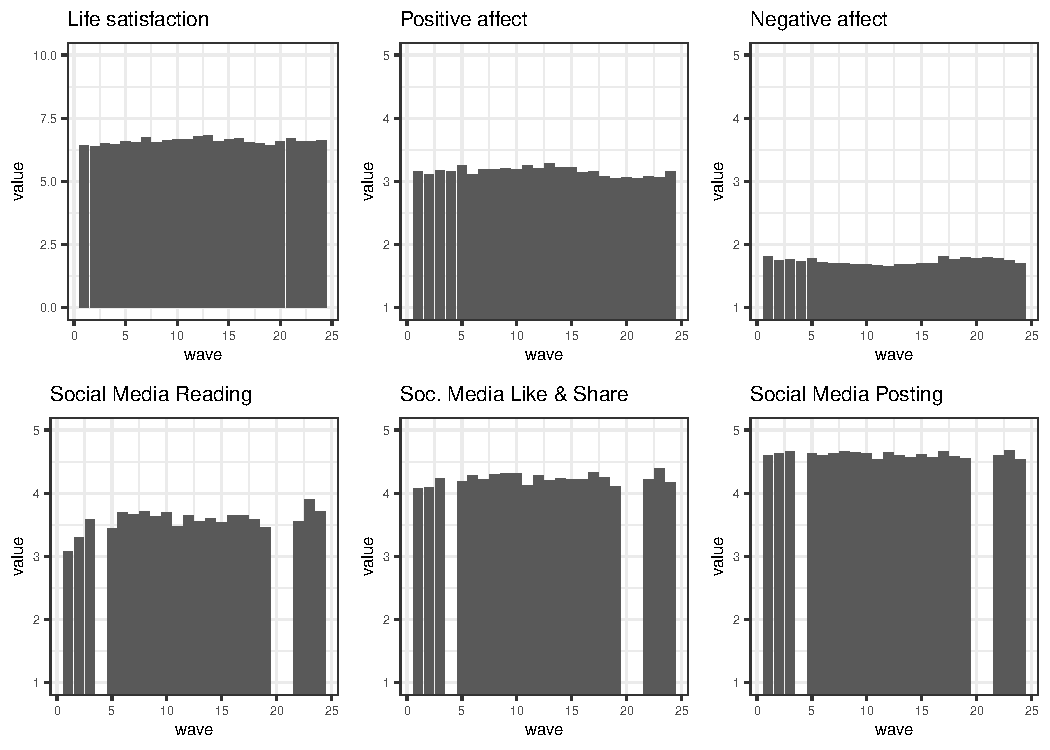
\includegraphics[width=\textwidth]{figures/fig_descriptives} \caption{Development of well-being and media use measures across the pandemic. Values obtained from mixed effect models, with participants and waves as grouping factors and without additional predictors.}\label{fig:fig-desc}
\end{figure}

The study's hypothesis was that the effects of social media use on well-being would be trivial.
Regarding the effects of different \emph{types} of communication---that is, reading vs.~sharing vs.~posting---all within-person effects fell completely within the a-priori defined SESOIs (see Figure \ref{fig:res-activity}).
For example, respondents who used social media more frequently than usual to read about COVID-19 related topics did not show a simultaneous change in life satisfaction (\emph{b} = 0.04 {[}95\% CI -0.02, 0.09{]}).
All confidence intervals include zero; hence, all effects were also statistically non-significant.
As a result, the hypothesis was supported for all COVID-19 related types of social media communication.

\begin{figure}
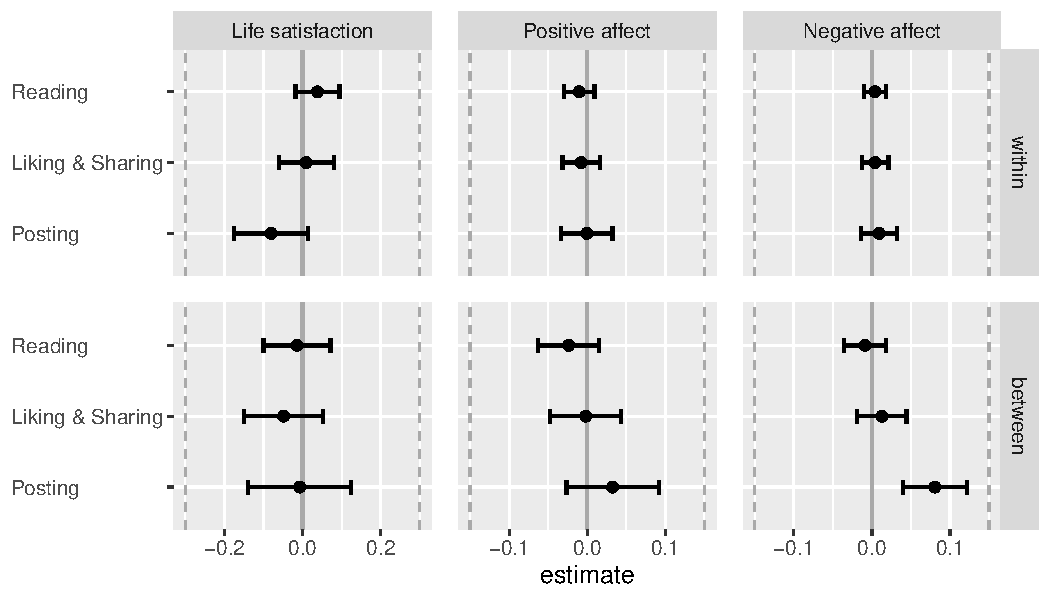
\includegraphics[width=\textwidth]{figures/fig_results_activity} \caption{The effects of various types of social media use on three indicators of well-being. Effects are controlled for a large number of covariates (see text). The SESOI was |0.30| for life satisfaction and |0.15| for affects. Hence, none of the reported effects are considered meaningful.}\label{fig:res-activity}
\end{figure}

Regarding between-person relations, about which no hypotheses were formulated, only one effect didn't include zero.
Respondents who across all waves used social media more frequently than others to write COVID-19 related posts reported higher levels of negative affect than others (\emph{b} = 0.08 {[}95\% CI 0.04, 0.12{]}).
The effect was still completely inside of the null region, hence not considered large enough to be practically relevant.

\begin{figure}
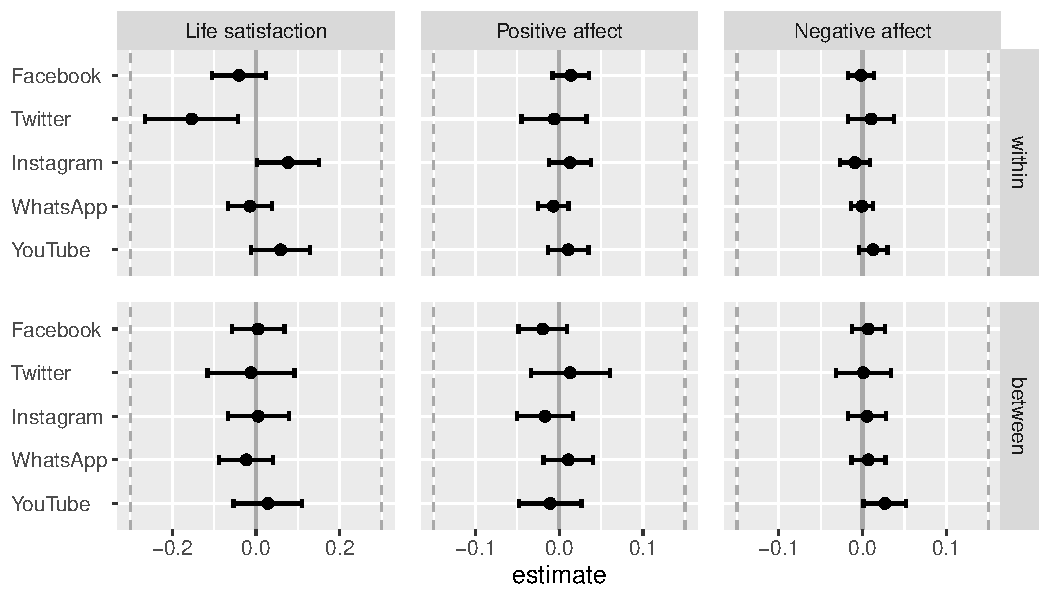
\includegraphics[width=\textwidth]{figures/fig_results_channel} \caption{The effects of using various social media applications on three indicators of well-being. Effects are controlled for a large number of covariates (see text). The SESOI was |0.30| for life satisfaction and |0.15| for affects. Hence, none of the reported effects are considered meaningful.}\label{fig:res-channels}
\end{figure}

Regarding the COVID-19 related use of social media \emph{channels}, the results were very comparable (see Figure \ref{fig:res-channels}).
Changes in the frequency of using different social media channels to attain information regarding COVID-19 were unrelated to meaningful changes in well-being.
For example, respondents who used Facebook more frequently than usual to learn about COVID-19 did not show a simultaneous change in well-being (\emph{b} = -0.04 {[}95\% CI -0.1, 0.02{]}).
Only two effects differed substantially from zero.
Respondents who used Instagram more frequently than usual to attain COVID-19 related news reported slightly higher simultaneous levels of life satisfaction than usual (\emph{b} = 0.08 {[}95\% CI \textless{} 0.01, 0.15{]}).
Respondents who used Twitter more frequently than usual to attain COVID-19 related news reported somewhat lower simultaneous levels of life satisfaction than usual (\emph{b} = -0.15 {[}95\% CI -0.27, -0.04{]}).
However, both effects were still completely inside of the null region, hence not considered large enough to be meaningful.
In sum, the hypothesis was supported also for the COVID-19 related use of important social media channels.

In terms of between-person relations---which, again, weren't included in the hypotheses---no relations crossed the null region or fell outside of it.
Only one relation did not include zero, was hence statistically significant.
Respondents who across all waves used YouTube more frequently than others for COVID-19 related reasons reported marginally higher levels of negative affect (\emph{b} = 0.03 {[}95\% CI \textless{} 0.01, 0.05{]}).
However, please note that this effect again was not considered large enough to be practically relevant.

\hypertarget{exploratory-analyses}{%
\subsection{Exploratory Analyses}\label{exploratory-analyses}}

In what follows, I briefly report also the results of some covariates.
Several variables showed larger associations with well-being.
Note because each variable has a different scaling, we would again need to define a SESOI for each variable, which cannot be implemented here.
But note that several variables would likely fall outside of such a SESOI.
This includes for example internal locus of control, health, or employment.
For a brief overview, see Figure \ref{fig:res-control}.

\begin{figure}
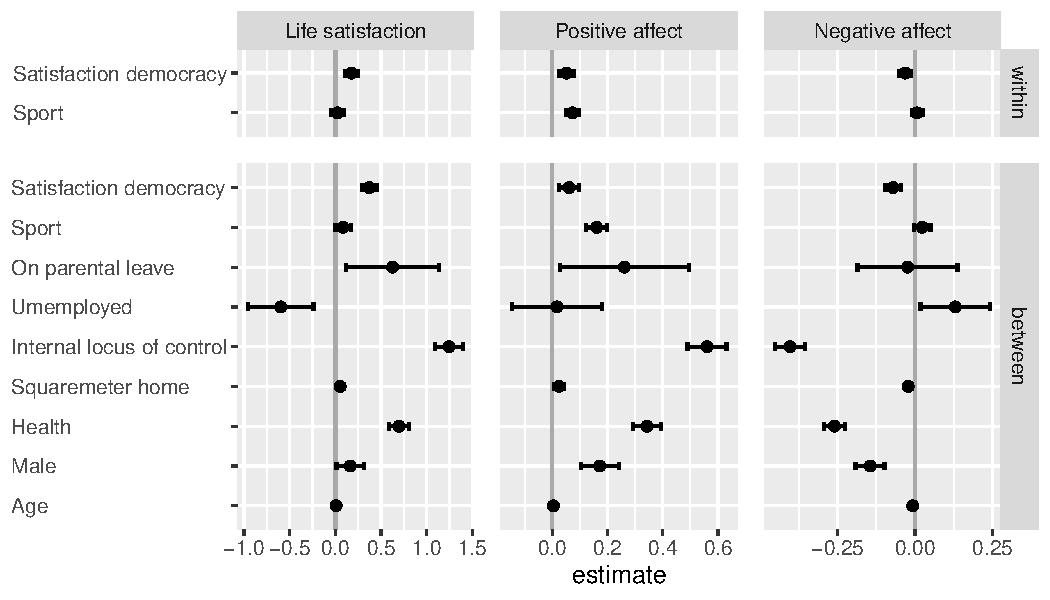
\includegraphics[width=\textwidth]{figures/fig_results_control} \caption{Results of selected covariates.}\label{fig:res-control}
\end{figure}

\hypertarget{discussion}{%
\section{Discussion}\label{discussion}}

In this study I analyzed the effects of COVID-19 related social media use on well-being.
The data come from a panel study with 24 waves and is representative of the Austrian population.
A random effects model, which separated between person relations from within-person effects and which controlled for several third variables, showed that within-person effects were trivial.
People who used social media more than usual to learn about COVID-19 did not show changes in their well-being.

The results imply that COVID-19 related social media use does not seem to be particularly relevant for people's well-being.
Other factors among the third variables that were measured revealed larger effects or relations, implying that well-being is rather determined by aspects such as health, employment, or locus of control.
According to this study, popular fears that ``doomscrolling'' or overusing social media during times of crises do not seem to be justified.

The study is not aligned with several recent studies on this particular research question or closely related research questions.
This includes a study by Bendau et al. (2021), which showed negative relations between social media and well-being.
However, note that Bendau et al. (2021) analyzed cross-sectional data on a between-person level, while not controlling for third variables, which is not optimal for investigating causal effects.
At the same time, this study is well-aligned with recent studies and meta-analyses analyzing the effects of social media use from a more general perspective or that adopted a somewhat different angle.
These studies have found that the effects of various types of social media use on several well-being indicators are small at best, often too small to matter (Ferguson et al., 2021; Meier \& Reinecke, 2020; Orben, 2020), which echoes the results obtained here.

\hypertarget{limitations}{%
\subsection{Limitations}\label{limitations}}

The current study analyzed whether changes in media use were related to changes in well-being, while controlling for several potential confounds.
Together, this allows for a good perspective on potential causality.
That said, causality necessitates temporal order, and the cause needs to precede the effect.
Regarding media use, such effects often happen immediately or shortly after use, necessitating intervals in the hours, minutes, or even seconds.
In many cases only experience sampling studies that ask users in the very moment can produce such knowledge.
However, even then we don't know for certain if we actually measured the right interval.
Hence, to document how effects unfold, future research needs to employ different study designs probing different time lags.
In addition, more thought needs to be invested in what relevant stable and varying factors should be selected as control variables.

Although I had already reduced the predefined SESOIs to be less conservative, potentially they were still too large.
Media use is only one aspect of several factors that simultaneously affect well-being.
Is it realistic that extremely changing only \emph{one} of these aspects (e.g., by completely stopping the use of social media) should already manifest in a detectable change in well-being?
Or would it make more sense to expect that if people regularly start doing say \emph{two} activities (e.g.~regularly exercising \emph{and} establishing a reading habit) together should show perceivable improvements to well-being?
In other words, the beneficial effect of a particular activity is large enough if people feel a difference when implementing two of those activities.
Practically, this would imply a SESOI half as large as I have defined here, that is \emph{b} = \textbar.15\textbar{} for well-being and \emph{b} = \textbar.075\textbar.
In this case, this would not make a difference, as even with these more liberal thresholds all but one effect would still be completely in the null region.
However, at all events future research needs to start a thorough discussion on what effect sizes are considered meaningful and relevant, and with this study I hope to provide some helpful input and first concrete guidelines.

Both media use and well-being were measured using self-reports.
Measuring well-being with self-reports is adequate, because it by definition requires introspection.
However, it would be preferable to measure social media use objectively, because people cannot reliably estimate their use.
That said, objective measures often cannot capture the content or the motivation of the use, and only very complicated tools that record the content that was used (such as the Screenome project) might produce such data.
Unfortunately, such procedures introduce other problems, for example related to privacy.
Hence, for this type of research question it seems necessary still to use self-reported measures.

Because the data were collected in a single country, the generalizability of the results is limited.
The results potentially apply primarily to the more Western sphere, and might not hold true in other cultures, especially cultures with a different media landscape or alternative social media channels.
That said, because this is a comparatively large study representative of a country's entire population, and because several waves were collected across a large time span, the results should be at least as generalizable as other typical empirical studies collected in the social sciences.

\hypertarget{conclusion}{%
\subsection{Conclusion}\label{conclusion}}

In this study, COVID-19 related social media use did not causally affect several indicators of well-being, including life satisfaction, positive affect, and negative affect.
However, factors other than social media use were more meaningfully related to well-being, such as physical health, employment, or believing that one is in control of one's life.
If it's the aim to improve well-being, it might hence be fruitful not to focus on social media but to address other, potentially more pressing societal problems related to inequality, safe spaces, or health care.

\newpage

\hypertarget{references}{%
\section{References}\label{references}}

\hypertarget{refs}{}
\begin{CSLReferences}{1}{0}
\leavevmode\hypertarget{ref-baguleyStandardizedSimpleEffect2009}{}%
Baguley, T. (2009). Standardized or simple effect size: {What} should be reported? \emph{British Journal of Psychology}, \emph{100}(3), 603--617. \url{https://doi.org/10.1348/000712608X377117}

\leavevmode\hypertarget{ref-bellFixedRandomEffects2019}{}%
Bell, A., Fairbrother, M., \& Jones, K. (2019). Fixed and random effects models: Making an informed choice. \emph{Quality \& Quantity}, \emph{53}(2), 1051--1074. \url{https://doi.org/10.1007/s11135-018-0802-x}

\leavevmode\hypertarget{ref-bendauAssociationsCOVID19Related2021}{}%
Bendau, A., Petzold, M. B., Pyrkosch, L., Mascarell Maricic, L., Betzler, F., Rogoll, J., \ldots{} Plag, J. (2021). Associations between {COVID}-19 related media consumption and symptoms of anxiety, depression and {COVID}-19 related fear in the general population in {Germany}. \emph{European Archives of Psychiatry and Clinical Neuroscience}, \emph{271}(2), 283--291. \url{https://doi.org/10.1007/s00406-020-01171-6}

\leavevmode\hypertarget{ref-beyensSocialMediaUse2021}{}%
Beyens, I., Pouwels, J. L., Driel, I. I. van, Keijsers, L., \& Valkenburg, P. M. (2021). Social {Media} {Use} and {Adolescents}' {Well}-{Being}: {Developing} a {Typology} of {Person}-{Specific} {Effect} {Patterns}. \emph{Communication Research}. \url{https://doi.org/10.31234/osf.io/ftygp}

\leavevmode\hypertarget{ref-choiMediatedCommunicationMatters2021}{}%
Choi, M., \& Choung, H. (2021). Mediated communication matters during the {COVID}-19 pandemic: {The} use of interpersonal and masspersonal media and psychological well-being. \emph{Journal of Social and Personal Relationships}, \emph{38}(8), 2397--2418. \url{https://doi.org/10.1177/02654075211029378}

\leavevmode\hypertarget{ref-cohenPowerPrimer1992}{}%
Cohen, J. (1992). A power primer. \emph{Psychological Bulletin}, \emph{112}(1), 155--159. \url{https://doi.org/10.1037/0033-2909.112.1.155}

\leavevmode\hypertarget{ref-dienerAdvancesOpenQuestions2018}{}%
Diener, E., Lucas, R. E., \& Oishi, S. (2018). Advances and open questions in the science of subjective well-being. \emph{Collabra: Psychology}, \emph{4}(1), 15. \url{https://doi.org/10.1525/collabra.115}

\leavevmode\hypertarget{ref-dienesUsingBayesGet2014}{}%
Dienes, Z. (2014). Using {Bayes} to get the most out of non-significant results. \emph{Frontiers in Psychology}, \emph{5}. \url{https://doi.org/10.3389/fpsyg.2014.00781}

\leavevmode\hypertarget{ref-dienlinImpactDigitalTechnology2020}{}%
Dienlin, T., \& Johannes, N. (2020). The impact of digital technology use on adolescent well-being. \emph{Dialogues in Clinical Neuroscience}, \emph{22}(2), 135--142. \url{https://doi.org/doi:10.31887/DCNS.2020.22.2/tdienlin}

\leavevmode\hypertarget{ref-edenMediaCopingCOVID192020}{}%
Eden, A. L., Johnson, B. K., Reinecke, L., \& Grady, S. M. (2020). Media for {Coping} {During} {COVID}-19 {Social} {Distancing}: {Stress}, {Anxiety}, and {Psychological} {Well}-{Being}. \emph{Frontiers in Psychology}, \emph{11}, 577639. \url{https://doi.org/10.3389/fpsyg.2020.577639}

\leavevmode\hypertarget{ref-fergusonThisMetaanalysisScreen2021}{}%
Ferguson, C. J., Kaye, L. K., Branley-Bell, D., Markey, P., Ivory, J. D., Klisanin, D., \ldots{} Wilson, J. (2021). Like this meta-analysis: {Screen} media and mental health. \emph{Professional Psychology: Research and Practice}. \url{https://doi.org/10.1037/pro0000426}

\leavevmode\hypertarget{ref-funderEvaluatingEffectSize2019}{}%
Funder, D. C., \& Ozer, D. J. (2019). Evaluating effect size in psychological research: {Sense} and nonsense. \emph{Advances in Methods and Practices in Psychological Science}, \emph{2}(2), 156--168. \url{https://doi.org/10.1177/2515245919847202}

\leavevmode\hypertarget{ref-greenspoonIntegrationSubjectiveWellbeing2001}{}%
Greenspoon, P. J., \& Saklofske, D. H. (2001). Toward an integration of subjective well-being and psychopathology. \emph{Social Indicators Research}, \emph{54}(1), 81--108. \url{https://doi.org/10.1023/A:1007219227883}

\leavevmode\hypertarget{ref-huangTimeSpentSocial2017}{}%
Huang, C. (2017). Time spent on social network sites and psychological well-being: {A} meta-analysis. \emph{Cyberpsychology, Behavior and Social Networking}, \emph{20}(6), 346--354. \url{https://doi.org/10.1089/cyber.2016.0758}

\leavevmode\hypertarget{ref-johannesNoEffectDifferent2021}{}%
Johannes, N., Dienlin, T., Bakhshi, H., \& Przybylski, A. K. (2021). \emph{No effect of different types of media on well-being}. PsyArXiv. \url{https://doi.org/10.31234/osf.io/zgb5y}

\leavevmode\hypertarget{ref-kerestesAdolescentsOnlineSocial2020}{}%
Keresteš, G., \& Štulhofer, A. (2020). Adolescents' online social network use and life satisfaction: {A} latent growth curve modeling approach. \emph{Computers in Human Behavior}, \emph{104}, 106187. \url{https://doi.org/10.1016/j.chb.2019.106187}

\leavevmode\hypertarget{ref-kittelAustrianCoronaPanel2020}{}%
Kittel, B., Kritzinger, S., Boomgaarden, H., Prainsack, B., Eberl, J.-M., Kalleitner, F., \ldots{} Schlogl, L. (2020). \emph{Austrian {Corona} {Panel} {Project} ({SUF} edition)}. AUSSDA. \url{https://doi.org/10.11587/28KQNS}

\leavevmode\hypertarget{ref-kittelAustrianCoronaPanel2021}{}%
Kittel, B., Kritzinger, S., Boomgaarden, H., Prainsack, B., Eberl, J.-M., Kalleitner, F., \ldots{} Schlogl, L. (2021). The {Austrian} {Corona} {Panel} {Project}: Monitoring individual and societal dynamics amidst the {COVID}-19 crisis. \emph{European Political Science}, \emph{20}(2), 318--344. \url{https://doi.org/10.1057/s41304-020-00294-7}

\leavevmode\hypertarget{ref-kleinDarklySoothingCompulsion2021}{}%
Klein, J. (2021). \emph{The darkly soothing compulsion of 'doomscrolling'}. Retrieved from \url{https://www.bbc.com/worklife/article/20210226-the-darkly-soothing-compulsion-of-doomscrolling}

\leavevmode\hypertarget{ref-klinePrinciplesPracticeStructural2016}{}%
Kline, R. B. (2016). \emph{Principles and practice of structural equation modeling} (4th ed.). New York, NY: The Guilford Press.

\leavevmode\hypertarget{ref-mcelreathYesterdayClass2021}{}%
McElreath, R. (2021). Yesterday in class, ... {[}Tweet{]}. Retrieved from \url{https://twitter.com/rlmcelreath/status/1354786005996482563}

\leavevmode\hypertarget{ref-meierComputerMediatedCommunicationSocial2020}{}%
Meier, A., \& Reinecke, L. (2020). Computer-{Mediated} {Communication}, {Social} {Media}, and {Mental} {Health}: {A} {Conceptual} and {Empirical} {Meta}-{Review}. \emph{Communication Research}, 009365022095822. \url{https://doi.org/10.1177/0093650220958224}

\leavevmode\hypertarget{ref-normanInterpretationChangesHealthrelated2003}{}%
Norman, G., Sloan, J., \& Wyrwich, K. (2003). Interpretation of changes in health-related quality of life: {The} remarkable universality of half a standard deviation. \emph{Medical Care}, \emph{41}(5), 582--592. Retrieved from \url{Retrieved\%20from\%20http://www.jstor.org/stable/3768017}

\leavevmode\hypertarget{ref-orbenTeenagersScreensSocial2020}{}%
Orben, A. (2020). Teenagers, screens and social media: A narrative review of reviews and key studies. \emph{Social Psychiatry and Psychiatric Epidemiology}, \emph{55}(4), 407--414. \url{https://doi.org/10.1007/s00127-019-01825-4}

\leavevmode\hypertarget{ref-orbenSocialMediaEnduring2019}{}%
Orben, A., Dienlin, T., \& Przybylski, A. K. (2019). Social media's enduring effect on adolescent life satisfaction. \emph{Proceedings of the National Academy of Sciences of the United States of America}, \emph{116}(21), 10226--10228. \url{https://doi.org/10.1073/pnas.1902058116}

\leavevmode\hypertarget{ref-przybylskiDoesTakingShort2021a}{}%
Przybylski, A. K., Nguyen, T. T., Law, W., \& Weinstein, N. (2021). Does {Taking} a {Short} {Break} from {Social} {Media} {Have} a {Positive} {Effect} on {Well}-being? {Evidence} from {Three} {Preregistered} {Field} {Experiments}. \emph{Journal of Technology in Behavioral Science}, \emph{6}(3), 507--514. \url{https://doi.org/10.1007/s41347-020-00189-w}

\leavevmode\hypertarget{ref-przybylskiLargescaleTestGoldilocks2017}{}%
Przybylski, A. K., \& Weinstein, N. (2017). A large-scale test of the {Goldilocks} hypothesis. \emph{Psychological Science}, \emph{28}(2), 204--215. \url{https://doi.org/10.1177/0956797616678438}

\leavevmode\hypertarget{ref-rohrerThinkingClearlyCorrelations2018}{}%
Rohrer, J. M. (2018). Thinking clearly about correlations and causation: {Graphical} causal models for observational data. \emph{Advances in Methods and Practices in Psychological Science}, \emph{24}(2), 251524591774562. \url{https://doi.org/10.1177/2515245917745629}

\leavevmode\hypertarget{ref-sandstromDoomscrollingCOVIDNews2021}{}%
Sandstrom, G., Buchanan, K., Aknin, L., \& Lotun, S. (2021). Doomscrolling {COVID} news takes an emotional toll -- here's how to make your social media a happier place. Retrieved from \url{http://theconversation.com/doomscrolling-covid-news-takes-an-emotional-toll-heres-how-to-make-your-social-media-a-happier-place-170342}

\leavevmode\hypertarget{ref-scharkowHowSocialNetwork2020}{}%
Scharkow, M., Mangold, F., Stier, S., \& Breuer, J. (2020). How social network sites and other online intermediaries increase exposure to news. \emph{Proceedings of the National Academy of Sciences}, \emph{117}(6), 2761--2763. \url{https://doi.org/10.1073/pnas.1918279117}

\leavevmode\hypertarget{ref-schemerImpactInternetSocial2021}{}%
Schemer, C., Masur, P. K., Geiß, S., Müller, P., \& Schäfer, S. (2021). The {Impact} of {Internet} and {Social} {Media} {Use} on {Well}-{Being}: {A} {Longitudinal} {Analysis} of {Adolescents} {Across} {Nine} {Years}. \emph{Journal of Computer-Mediated Communication}, \emph{26}(1), 1--21. \url{https://doi.org/10.1093/jcmc/zmaa014}

\leavevmode\hypertarget{ref-stainbackCOVID1924News2020}{}%
Stainback, K., Hearne, B. N., \& Trieu, M. M. (2020). {COVID}-19 and the 24/7 {News} {Cycle}: {Does} {COVID}-19 {News} {Exposure} {Affect} {Mental} {Health}? \emph{Socius}, \emph{6}, 2378023120969339. \url{https://doi.org/10.1177/2378023120969339}

\leavevmode\hypertarget{ref-statistaAverageDailyTime2021}{}%
Statista. (2021). \emph{Average daily time spent on social networks by users in the {United} {States} from 2018 to 2022}. Retrieved from \url{https://www.statista.com/statistics/1018324/us-users-daily-social-media-minutes/}

\leavevmode\hypertarget{ref-waterlooNormsOnlineExpressions2018}{}%
Waterloo, S. F., Baumgartner, S. E., Peter, J., \& Valkenburg, P. M. (2018). Norms of online expressions of emotion: {Comparing} {Facebook}, {Twitter}, {Instagram}, and {WhatsApp}. \emph{New Media \& Society}, \emph{20}(5), 1813--1831. \url{https://doi.org/10.1177/1461444817707349}

\end{CSLReferences}

\newpage

\hypertarget{competing-interests}{%
\section{Competing Interests}\label{competing-interests}}

I declare no competing interests.

\hypertarget{supplementary-material}{%
\section{Supplementary Material}\label{supplementary-material}}

All the stimuli, presentation materials, analysis scripts, and a reproducible version of the manuscript can be found on the companion website (\url{https://xmtra.github.io/Austrian_Corona_Panel_Project/index.html}).

\hypertarget{data-accessibility-statement}{%
\section{Data Accessibility Statement}\label{data-accessibility-statement}}

The data are shared on AUSSDA, see \url{https://doi.org/10.11587/28KQNS}.
The data can only be used for scientific purposes.


\end{document}
